\documentclass{article}

% If you're new to LaTeX, here's some short tutorials:
% https://www.overleaf.com/learn/latex/Learn_LaTeX_in_30_minutes
% https://en.wikibooks.org/wiki/LaTeX/Basics

% Formatting
\usepackage[utf8]{inputenc}
\usepackage[margin=1in]{geometry}
\usepackage[titletoc,title]{appendix}

% Math
% https://www.overleaf.com/learn/latex/Mathematical_expressions
% https://en.wikibooks.org/wiki/LaTeX/Mathematics
\usepackage{amsmath,amsfonts,amssymb,mathtools}
\usepackage{subcaption}
% Images
% https://www.overleaf.com/learn/latex/Inserting_Images
% https://en.wikibooks.org/wiki/LaTeX/Floats,_Figures_and_Captions
\usepackage{graphicx,float}
\usepackage{subcaption}

% Tables
% https://www.overleaf.com/learn/latex/Tables
% https://en.wikibooks.org/wiki/LaTeX/Tables

% Algorithms
% https://www.overleaf.com/learn/latex/algorithms
% https://en.wikibooks.org/wiki/LaTeX/Algorithms
\usepackage[ruled,vlined]{algorithm2e}
\usepackage{algorithmic}

% Code syntax highlighting
% https://www.overleaf.com/learn/latex/Code_Highlighting_with_minted
\usepackage{minted}
\usemintedstyle{borland}

% References
% https://www.overleaf.com/learn/latex/Bibliography_management_in_LaTeX
% https://en.wikibooks.org/wiki/LaTeX/Bibliography_Management
\usepackage{biblatex}
\addbibresource{references.bib}

\title{Time-Scale Modification(TSM) on Audio Signals}
\author{Chuanmudi Qin, Tianqi Gu}
\date{Mar 19th, 2020}

\begin{document}

\maketitle

\begin{abstract}
    Time-scale modification(TSM) procedures are digital signal processing methods for stretching or compressing the duration of a given audio signal. Ideally, it should not change its content such as pitch and timbre. In this project we implement two algorithms based on Short Time Fourier Transform(STFT) to achieve TSM: Overlapping-add method(OLA) and Phase Vocoder(PV). 
\end{abstract}

\section{Overview and Introduction}
An audio file is usually composed of two elements, its data points, represented by an array $y$, and the sampling rate, represented by a natural number $Fs$. A common sampling rate is 44.1kHz, meaning that 44100 points are sampled per second. To adjust the play speed of an audio file, the simplest way is to multiply an coefficient $n$ to $Fs$, making it $n$ times faster or slower. However the frequencies of the original signal would be stretch by $n$ at the same time, changing its pitch and timbre.
\begin{figure}[H]
\centering        
\includegraphics[height=6.5cm, width=4cm]{images/youtube-playback-speed-options.jpg}
\caption{playback speed}
\end{figure}
\textcolor{red}{need pictures here.}\\
Therefore, to adjust the play speed without changing the original frequencies, we need to reconstruct an array of data of length $n$ times the original one, and preserve its frequency domain information. In the following sections, two algorithms are explored and discussed. The first one is a naive Overlapping-add(OLA) method and the second one is Phase Vocoder(PV) based on Short-Time Fourier Transform(STFT) and OLA.\\
We worked on two audio signals. The first one is a song named \textit{Medicine.wav} that is around 3 minutes long with sampling rate 44.1kHz. The second one is a audio sampled from Prof.Nathan Kutz's Amath 581 lecture, named as \textit{Cluster.wav}, which is around 2 minutes long with sampling rate 44.1kHz. And without loss of generality, in this project we focus on 2X acceleration of the play speed as an example.
\section{Theoretical Background}
\subsection{Notations}
\begin{itemize}
  \item $H_a$: analysis window hop size 
  \item $H_s$: synthesis window hop size
  \item $L$: window length, also the length of each section 
  \item $x_k(m)$ or $y_k(m)$: the m-th element of the k-th segment
\end{itemize}

\subsection{Overlapping Add(OLA)}
The main idea behind this method is  cutting the original time-domain signal into pieces and overlap them in order to achieve time scale modification.  \\
Cutting up the signal $x(n)$ is done with a window function $w(x)$ of length $L$. It can be thinking of either sliding the signal across the window centering at the origin: 
\begin{equation}
 x_{k}(n) =x(n+kH_a)w(n) 
\label{eq : }
\end{equation}
or sliding the window along the signal started from the origin: 

\begin{equation}
 x_{k}(n) =x(n)w(n-kH_a) 
\label{eq : }
\end{equation}
the windowed \textit{analysis frame} can be represented as: 
\begin{equation}
x_k(n) = \begin{cases}
        x(n +kH_a),  \text{\qquad if $n = 1,2,3,...,L$}\\
        0, \text{\qquad  \qquad \qquad otherwise} 
\end{cases}
\label{eq : }
\end{equation}
The \textit{synthesis frame} can be constructed by removing the effect of the window when overlapping as follow: 

\begin{equation}
        y_k(n) = \frac{x_{k}(n)}{\sum_{r\in \mathbb{Z}}^{\infty}w(n-rH_s) }
\label{eq : }
\end{equation}
After getting the frames, we need to stitch them together to get the time domain scaled signal: 
\begin{equation}
        y(n) =\sum_{k \in \mathbb{Z}} y_{k}(n - kH_s) \label{eq:}
\end{equation}
%\textcolor{red}{need pictures here: y(n)}
\subsection{STFT Analysis}
\subsubsection{Fourier Transform View of STFT:}
Discrete STFT is DFT on every segment of the input signal. In the context of TSM, we use a window function $w(x)$ to cut the signal. STFT analysis equation is the following:
\begin{equation}
        X(mH_a,k) = \sum_{n=0}^{n= N-1} x(n+mH_a) w(n) e^{2 \pi ik \frac{n}{N}} 
\end{equation}
window function in this context serves as a tapper function. In this project, hamming window 
\[
w(n) = sin^2\bigg(\frac{\pi n}{N} \bigg), \hspace{1cm} -N/2 \leq n \leq N/2
\]
is used instead of a rectangular window for two reasons. Firstly, DFT assumes the signal is periodic, hamming zeros signals out at the two ends to satisfy the periodicity avoiding introducing high frequency components. Secondly, hamming window is used to avoid spectrum leakage. Windows can be viewed as filters in frequency domain(explained in the following section). Due to that the frequency response of rectangular window has higher side-lobes, when convolving with the signal, it picks up more unwanted frequencies outside of the target frequency bin, which would lead to a noisy reconstruct signal. Although hamming window has lower side-lobes, it has a wider main lobe, which will lead to smearing(this is obvious when playing back at a lower speed). Hence there is a trade off between what kind of window to use.
\subsubsection{Filter Bank View of STFT:}
STFT can be viewed as a convolution.\\ 
\[
        \begin{aligned}
        X(mH_a,k) &= \sum_{n=0}^{n= N-1} x(n+mH_a) w(n) e^{2 \pi ik \frac{n}{N}}\\ 
                  &=\sum_{n=0}^{n=N-1}(x(n)e^{-i\omega_k n})w(n-mH_a)\\
                  &=  (x(n) e^{-i\omega_k n} )* w(n)
\end{aligned}
\]
where  $x(n) e^{-i\omega_k n}$ can be view as a modulation of $X(\omega)$\\
%\textcolor{red}{need pictures here: filter bank view}\\
the Filter Bank view enable us to interpret $X(m,k)$ as the frequency components of $x_m(n)$ on the channel where $\omega_k=\frac{2\pi k}{N}$ \\ 
Noticed that frequencies in this formula is also discretized given by $\omega_{k} = \frac{2\pi k}{N}$, $k=0,1,2...N-1$. Frequency resolution is determined once a window length is selected. The base band will be $\frac{2\pi}{N}$. The larger length of the window, the finer the frequency resolution. 
\subsection{STFT Synthesis:}
Between STFT analysis and STFT synthesis, there is a processing step, which in our project is done with phase vocoder. $X^{+}(m,k)$ is the modified signal after phase vocoder. Detailed phase vocoder is discussed in the next section. 
STFT synthesis: 
\begin{equation}
        y_k(n) = \frac{1}{N}\sum_{k=0}^{N-1} X^{+}(m,k) e^{\frac{2\pi i k n}{N}} 
\end{equation}
Noticed that our goal is Overlapping add, therefore another window function will be in used to smooth out the signal. At the end, we need to remove the effect of the window. The synthesis frame are derived as:
\begin{equation}
        y^{*}_k(n) = \frac{w(n)y_k(n)}{\sum_{m\in \mathbb{Z}}w(n-mH_s)^2}
\end{equation}
\subsubsection*{STFT OLA requirements:}
1. 50\% overlap to avoid information loss\\
2. bandwidth of the window HAS to be wider than than the base band. otherwise leads to loss of freq information\\
3. step/hop size

\subsection{Phase Vocoder(PV)}
From the Above , we get the Fourier coefficient of the k-th frequency bin of the m-th analysis frame in complex form: $ X_{m}[k] = a + bi$. Phase and angle can be calculated. \\
\[
\begin{aligned}
        |X_{m}[k]|=&A= \sqrt{a^2+b^2}  \\
        \angle X_{m}[k]=&\phi_{m}[k]= arctan\{\frac{b}{a}\} \\
\end{aligned}
\]
Another way of representing complex number is 
\begin{equation}
        X_m[k] = |X_m[k]| e^{i\phi_{m}[k]}
\label{eq : }
\end{equation}
Realizing that there is a difference between wrapped and unwrapped phase: a wrapped phase is always in the interval $[-\pi, \pi]$, whereas a unwrapped phase is not bounded.\\
Although we are trying to use fit all the frequencies at a specific DFT channel k, where $\omega_k = \frac{i2\pi k}{N}$, the phase of the signal at frequency $\omega_k$ at the end of one DFT segment may not align with the phase of signal at the same frequency at the start of the following DFT section(illustrated in figure). This would cause warbling artifact. There are many algorithms to achieve the phase adjustment. \\
If phase is unwrapped, then the true frequency can be recovered by $\omega = \frac{\phi_{unwrapped}}{\Delta t} $. However, given the FT coefficient, phases calculated from these coefficient is wrapped, which makes the estimation of the true phase complicated. \\
Approximating the true phase of the $m^{th}$ segment is done with $\tilde{\phi}_m[k] = \phi_{m-1} + \Delta t \omega_{true}$, where $\omega_{true}$ is unknown. To get this, Firstly, we need to calculate the unwrapped change in frequency $\Delta\omega_m[k]= \frac{\phi_m[k] - \phi_m[k-1]}{\Delta t} - \omega[k]$. Then wrap this frequency in $[-\pi, \pi]$ to get $\Delta\omega_{wrapped}$. Finally the approximation to the  $\omega_{true}[k]=\omega[k]+\omega_{wrapped}$\\
With the newly calculated  $\tilde{\phi}_m[k]$, I get the modified $\tilde{X}_m[k] = Ae^{i\tilde{\phi}_m[k] }$. Synthesis steps comes after this.


\section{Algorithm implementation and development }
\subsection{Choosing parameters:}
Window length: 8192 \\
overlapping factor: 0.75 \\
Analysis hop size: 2048\\
Synthesis hop size: 4096\\
stretch factor: 2
\subsection{Phase Vocoder with STFT: }
1. Utilize python fft in numpy package to transform every windowed 8192 points as one segment.  \\
2. Using phase vocoder algorithm to make correction on each of the segments. This is a iterative process.  \\
3. Keep track of at each point, the accumulative window weights.\\
4. Use ifft transform the modified segments back.\\
5. Apply the synthesis window to each of the segments and factor out the sum of window weights every single points. \\
6. Overlapping add the synthesis frames to get the reconstructed signal.


\section{Computational Result}
When processing the signals, we fine tuned the parameters to make the modified audio sounds good. The parameters we finally choose for OLA and PV are: window length = 8192, overlap factor = 0.5 and stretch factor = 0.5. If we make the Hamming window to narrow, the processed audios will be significantly off tune, and if we take too big hop size, there will be discontinuity and thus loss of information.
Ideally, when accelerate the play speed to 2X, the time domain signal is compressed horizontally. And since we want to preserve the original pitch and timbre, the distribution in frequency domain stay the same shape.\\
Figure 2 and 3 show the original time domain and frequency domain signals for both audio files. Figure 3 and 4 show the time scaled modified signals by OLA in time and frequency domain. Figure 5 and 6 show the time scale modified signals by PV in time and frequency domain. \\
By comparing these three groups of signals, we can tell that both OLA and PV have done their jobs. It is hard to notice any difference between signals modified and PV modified signals just by comparing results in Figure 3 and Figure 4. Both results have smaller amplitude comparing to the original signals, and the amplitude of signals obtained by PV is smaller than that obtained by OLA. \\
Signals modified by OLA are expected to have distortion due to phase jumps, which results into clicks corresponding to high frequency components, while signals modified by PV does not have this defect. By comparing Figure 3 and 4 we can find that in frequency domain PV modified signals are closer to the original signals, especially for music file \textit{Medicine.wav}, while OLA modified signals seems to have a little bit information loss and high frequency noise. Nevertheless, the differences are hard to notice.\\
We wrote an iPython Notebook in the Github page to enable us to listen to the modified signals. Since we fine tuned the parameters window length, stretch factor and overlap factor, those signals modified by OLA and PV sounds quite similar, except audio files processed by PV sounds smoother. 
\begin{figure}[h!]
\centering
    \begin{subfigure}{0.45\textwidth}
      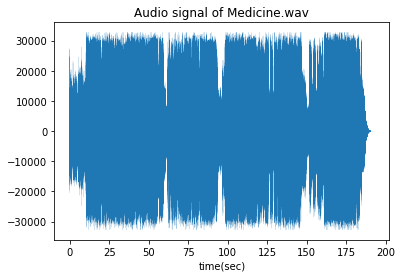
\includegraphics[width=\textwidth]{Medicine_original.png}
    \end{subfigure}%
    \begin{subfigure}{0.45\textwidth}
      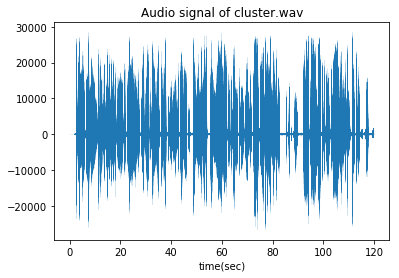
\includegraphics[width=\textwidth]{Cluster_original.png}
    \end{subfigure}
    \begin{subfigure}{0.45\textwidth}
      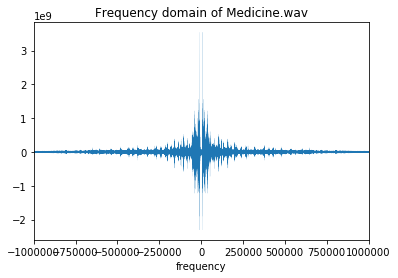
\includegraphics[width=\textwidth]{Medicine_freq.png}
    \end{subfigure}%
    \begin{subfigure}{0.45\textwidth}
      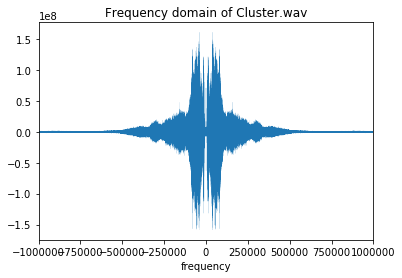
\includegraphics[width=\textwidth]{Cluster_freq.png}
    \end{subfigure}
    \caption{Original audio files in time and frequency domain}
    \label{fig:mylabel}
\end{figure}

\begin{figure}[h!]
\centering
    \begin{subfigure}{0.45\textwidth}
      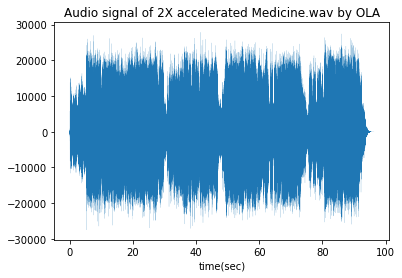
\includegraphics[width=\textwidth]{Medicine_2X_OLA.png}
    \end{subfigure}%
    \begin{subfigure}{0.45\textwidth}
      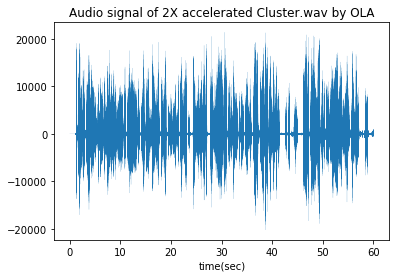
\includegraphics[width=\textwidth]{Cluster_2X_OLA.png}
    \end{subfigure}
    \begin{subfigure}{0.45\textwidth}
      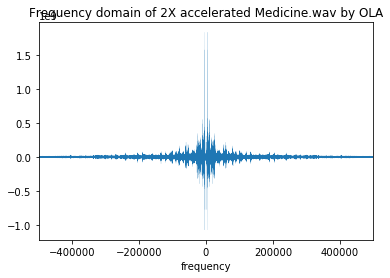
\includegraphics[width=\textwidth]{Medicine_2X_OLA_freq.png}
    \end{subfigure}%
    \begin{subfigure}{0.45\textwidth}
      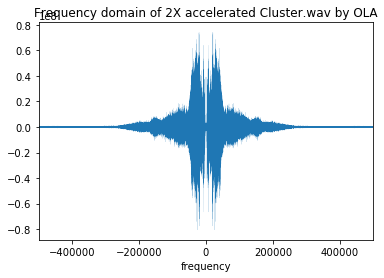
\includegraphics[width=\textwidth]{Cluster_2X_OLA_freq.png}
    \end{subfigure}
    \caption{Audio files after 2X accelerated by OLA in time and frequency domain}
    \label{fig:mylabel}
\end{figure}

\begin{figure}[h!]
\centering
    \begin{subfigure}{0.45\textwidth}
      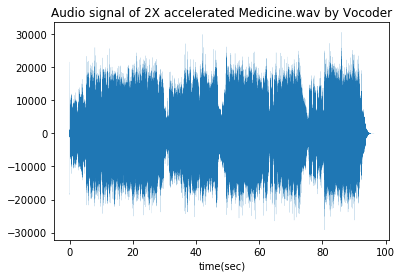
\includegraphics[width=\textwidth]{Medicine_2X_Vocoder.png}
    \end{subfigure}%
    \begin{subfigure}{0.45\textwidth}
      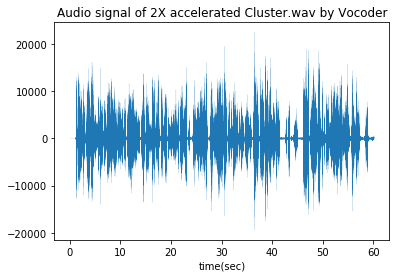
\includegraphics[width=\textwidth]{Cluster_2X_Vocoder.png}
    \end{subfigure}
    \begin{subfigure}{0.45\textwidth}
      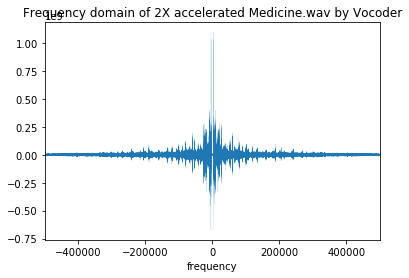
\includegraphics[width=\textwidth]{Medicine_2X_Vocoder_freq.png}
    \end{subfigure}%
    \begin{subfigure}{0.45\textwidth}
      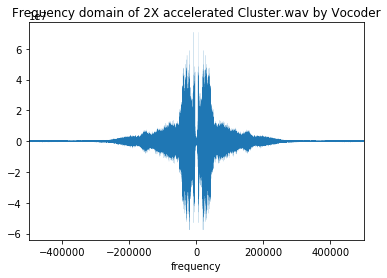
\includegraphics[width=\textwidth]{Cluster_2X_Vocoder_freq.png}
    \end{subfigure}
    \caption{Audio files after 2X accelerated by Vocoder in time and frequency domain}
    \label{fig:mylabel}
\end{figure}

\newpage

\section*{Conclusion and Summary}
In conclusion, we find that Phase Vocoder(PV) is a better way to implement time-scale modification on audio signals, but if we fine tune parameters, OLA can work almost as well as PV. Even though in this project we take 2X acceleration as an example, by adjust parameters in the iPython notebook, we can easily accelerate or decelerate the file by any rate.\\
Meanwhile, there are some interesting problems we haven't explored yet. How did the parameters affect the modified signal's pitch and timbre numerically? Given a audio signal how to determine the best parameters analytically without tuning them by hand?


\newpage
\section*{Appendix A: Python Code }
GITHUB: : \href{https://github.com/mumudididi/Amath582FinalProject}

\begin{minted}[
frame=lines,
framesep=2mm,
baselinestretch=1.2,
fontsize=\footnotesize,
linenos
]
{Python}
dir()
for name in dir():
    if not name.startswith('_'):
        del globals()[name]

import math
import sounddevice as sd
from scipy.io import wavfile
import matplotlib.pyplot as plt
import numpy as np
import cmath

fs, data = wavfile.read('Medicine.wav')
fs, data = wavfile.read('Cluster.wav')
data =data[:,0]

time = np.arange(len(data))
plt.plot(time/fs, data, linewidth=0.1)
plt.xlabel('time(sec)')
plt.title('Audio signal of Medicine.wav')
plt.show()

data_freq = np.fft.fft(data)
data_freq = np.fft.fftshift(data_freq)
n = int(len(data_freq)/2)
freq = np.arange(-n,n,1)
plt.plot(freq, data_freq, linewidth=0.1)
plt.xlabel('frequency')
plt.title('Frequency domain of Cluster.wav')
plt.xlim((-1000000,1000000))
plt.show()

sd.play(data,fs)
sd.stop()

def padding(data,window_len,hop_size,Ahop_times):
    #Ahop_times = int(np.ceil((len(data) - window_len)/hop_size))
    required_len = int(hop_size * (Ahop_times)+window_len)
    pad_len = required_len - len(data)
    #return [required_len,pad_len,np.append(data,np.zeros(pad_len))]
    return [pad_len,np.append(data,np.zeros(pad_len))]
    
def init_analysis_hop(data, window_len,overlap_factor):
    length_of_original = len(data)
    overlap_length= overlap_factor * window_len
    Analysis_H = (1-overlap_factor) * window_len
    #Ahop_times = round(length_of_original/ Analysis_H) -1
    Ahop_times = int(np.ceil((length_of_original - window_len)/Analysis_H))
    newData = padding(data, window_len,Analysis_H,Ahop_times)
    gama = Analysis_H * np.arange(0,Ahop_times+1)
    return [Ahop_times, gama, newData[0],newData[1]]

def analysis_slice(data, Ahop_times, gama,window_len):
    window = np.hamming(window_len)
    transformed_xw=[]
    for start_point in gama:
        start_point =int(start_point)
        xw =np.multiply(data[start_point:start_point+window_len],window)
        transformed_xw = transformed_xw + [np.fft.fft(xw)]
    print(len(transformed_xw))
    return transformed_xw

def init_synthesis_hop(stretch_factor,window_len,gama,transformed_xw):
    beta = stretch_factor*gama
    rec_len =int( beta[-1]+ window_len)
    windowSum = np.zeros(rec_len)
    ola_sig= np.zeros(rec_len)
    winSquare =np.multiply(np.hamming(window_len),np.hamming(window_len))
    ind= 0;
    for start in beta:
        start=int(start)
        windowSum[start: start+window_len] = windowSum[start:start+window_len] +  winSquare
        ola_sig[start:start+window_len] = ola_sig[start:start+window_len]+ np.multiply(np.fft.ifft(transformed_xw[ind]),np.hamming(win_len))
        ind=ind+1
    recSig = np.divide(ola_sig,windowSum)
    return [beta, rec_len,recSig]
    
def vocoder(stretch_factor,fs,win_len,overlap_factor,trans_xw):
    ratio = stretch_factor
    X_tilta = [] 
    diff=[]
    delta_freq_coarse = np.arange(0,win_len)* fs/win_len 
    delT = (1-overlap_factor)*win_len /fs
    phi_prev = np.zeros(win_len) 
    phi_acc = np.zeros(win_len)
    delt_s= ratio * delT
    for arr in trans_xw:
      current_p =np.angle(arr)
      current_A=np.abs(arr)
      delta_phi = (current_p - phi_prev)/delT -delta_freq_coarse;
      delta_phi_wrapped = np.mod(delta_phi+math.pi, 2*math.pi)-math.pi
      omega_true = delta_freq_coarse + delta_phi_wrapped
      phi_acc   = phi_prev +omega_true*delt_s
      phi_prev = current_p
      X_tilta = X_tilta + [np.multiply(current_A,np.exp(1j*phi_acc))]
    return X_tilta

#### STFT OLA##########

win_len = 8192
overlap_factor =0.5
stretch_factor = 0.5
[Ahop_times,gama,pad_len,newData] = init_analysis_hop(data,win_len, overlap_factor=overlap_factor)
trans_xw= analysis_slice(newData,Ahop_times,gama,win_len)
[beta, rec_len,recSig]=init_synthesis_hop(stretch_factor=stretch_factor,window_len=win_len,gama=gama,transformed_xw=trans_xw)

#### STFT Phase Vocoder##########

win_len = 8192
overlap_factor =0.5
stretch_factor = 0.5
[Ahop_times,gama,pad_len,newData] = init_analysis_hop(data,win_len, overlap_factor=overlap_factor)
trans_xw= analysis_slice(newData,Ahop_times,gama,win_len)
trans_xw= vocoder(stretch_factor ,fs,win_len,overlap_factor,trans_xw)
[beta, rec_len,recSig]=init_synthesis_hop(stretch_factor=stretch_factor,window_len=win_len,gama=gama,transformed_xw=trans_xw)

sd.play(np.int16(recSig),fs)
sd.stop()

time = np.arange(len(recSig))
plt.plot(time/fs, np.int16(recSig), linewidth=0.1)
plt.xlabel('time(sec)')
plt.title('Audio signal of 2X accelerated Cluster.wav by Vocoder')
plt.show()

data_freq = np.fft.fft(np.int16(recSig))
data_freq = np.fft.fftshift(data_freq)
n = int(len(data_freq)/2)
freq = np.arange(-n,n,1)
plt.plot(freq, -data_freq, linewidth=0.1)
plt.xlabel('frequency')
plt.title('Frequency domain of 2X accelerated Cluster.wav by Vocoder')
plt.xlim((-500000,500000))
plt.show()
\end{minted}


\section*{Bibliography}
\end{document}

\section{Chapter 1}
\subsection*{Problem 1}

\begin{enumerate}[label=\roman*)]
  \item $a \in \Z$
  \item $A^\Trans = A$
  \item $A\vec{v} = \lambda \vec{v}$
  \item $\One$
\end{enumerate}
pupupu $|a|=15$, pupupupu.
